\documentclass[10pt,twocolumn,letterpaper]{article}

\usepackage{cvpr}
\usepackage{times}
\usepackage{epsfig}
\usepackage{graphicx}
\usepackage{amsmath}
\usepackage{amssymb}

\cvprfinalcopy

\def\cvprPaperID{****}
\def\httilde{\mbox{\tt\raisebox{-.5ex}{\symbol{126}}}}

% Pages are numbered in submission mode, and unnumbered in camera-ready
\ifcvprfinal\pagestyle{empty}\fi
\begin{document}

%%%%%%%%% TITLE
\title{M5 Forecasting - Accuracy: Estimate the unit sales of Walmart retail goods}

\author{Flavio Amurrio-Moya\\
George Mason University\\
4400 University Dr, Fairfax, VA 22030\\
{\tt\small famurrio@gmu.edu}
\and
Pyoung Kang Kim\\
George Mason University\\
4400 University Dr, Fairfax, VA 22030\\
{\tt\small pkim23@gmu.edu}
}

\maketitle
\thispagestyle{empty}

%%%%%%%%% ABSTRACT
\begin{abstract}
% Problem, gap, approach, key results
  Methods based on decision trees dominate the field of tabular regressional
  problems and have shown to outperform many other methods, such as weighted
  averaging and other outperforming methods that are natively time-series based
  on using networks such as LSTM/GRU. In this report, we plan to test out a pure
  Deep Learning approach which leverages key foundational concepts in both
  supervised and unsupervised learning to attempt to reach an acceptable score
  with minimum data manipulation, and virtually no data gathering and/or
  wrangling.

  The ``M5 Forecasting - Accuracy: Estimate the unit sales of Walmart retail
  goods'' competition (which will be referred to as the ``M5 Forecasting
  Competition'' and/or ``The Competition'') challenged Kaggle users to design a
  learning model that would be able to predict how many of a certain item would
  be sold on a given day. In this paper, we embark on the challenge to create
  such a model and improve on current strategies.

\end{abstract}

%%%%%%%%% BODY TEXT
\section{Introduction}
% Broad problem and impact
% scientific gap(what technical aspects have not yet been solved)
% summary approach (should include reference to technical gap)
% key results
The M5 Forecasting competition was created on Kaggle by ``The Makridakis Open
Forecasting Center (MOFC) at the University of Nicosia''. This was done with the
intent of being able to forecast the sales of items in order to minimize
opportunity loss (such as not having enough of an item in stock) as well as to
avoid stocking too much of an unpopular item. This competition aims to achieve
more accurate and better-calibrated forecasts, reduce waste, and be able to
appreciate uncertainty and its risk implications. \cite{kaggle}

In this paper, we discuss an approach to tabular regressional learning that is
an end to end Deep Learning solution. We try various modifications to the
network and it's loss function and discuss key points that will help achieve
higher scores during the competition.

We were provided with hierarchical sales data from Walmart to forecast daily
sales for the next 28 days. The data covers stores in three US states
(California, Texas, and Wisconsin) and includes item level, department, product
categories, and store details. It also contains explanatory variables such as
price, promotions, day of the week, and special events.



\subsection{Data}
  We were given a dataset that contained 3 CSV files to be
  used for training.\cite{kaggle}

  \noindent {\bf calendar.csv} - information regarding dates of product sales.
{\small\begin{verbatim}
schema: date, wm_yr_wk, weekday, wday, month,
        year, d, event_name_1, event_type_1,
        event_name_2, event_type_2, snap_CA,
        snap_TX, snap_WI

row: 2011-01-29, 11101, Saturday, 1, 1, 2011,
     d_1, , , , , 0 , 0 , 0
\end{verbatim}}

  % \noindent schema - date, wm\_yr\_wk, weekday, wday, month, year, d, event\_name\_1,
  % event\_type\_1, event\_name\_2, event\_type\_2, snap\_CA, snap\_TX, snap\_WI

  % \noindent row - 2011-01-29, 11101, Saturday, 1, 1, 2011, d\_1, , , , , 0 , 0 , 0


  \noindent {\bf sales\_train\_validation.csv} - actual sales respective to date ‘d’, by hierarchical data.
  {\small\begin{verbatim}
schema: id, item_id, dept_id, cat_id,
        store_id, state_id, d_1,...d_1913

row: HOBBIES_1_001_CA_1_validation,
     HOBBIES_1_001, HOBBIES_1, HOBBIES,
     CA_1, CA, 0, ...1
  \end{verbatim}}


  \noindent {\bf sell\_prices.csv} - prices of products per a certain store and date

  {\small\begin{verbatim}
schema: store_id, item_id, wm_yr_wk, sell_price

row: CA_1, HOBBIES_1_001, 11325, 9.58
  \end{verbatim}}



\subsection{Closer Look At The Data}
  Graphing the data allows us to visualize some of the shopping trends.

\begin{figure*}
  \begin{center}
    % \fbox{\rule{0pt}{2in} \rule{.9\linewidth}{0pt}}
    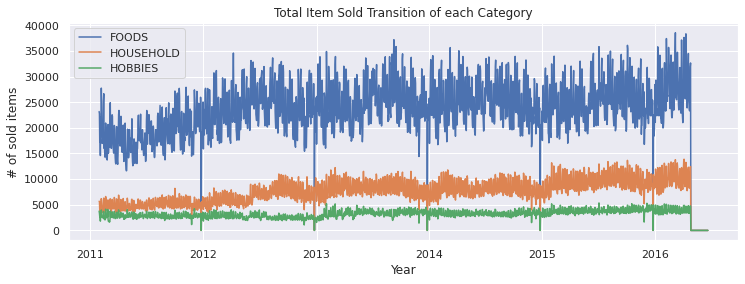
\includegraphics[width=0.8\linewidth]{img/totalItemSoldofEachCategory.png}
  \end{center}
  \caption{Total items sold of each category.\cite{ryuheeeei_2020}}
  \label{fig:totalItemSoldofEachCategory}
\end{figure*}
  In Figure~\ref{fig:totalItemSoldofEachCategory} we can visualize the number of
  items per category. We can see a certain drop towards the end of each year
  which we'll see in later graphs.

\begin{figure*}
  \begin{center}
    % \fbox{\rule{0pt}{2in} \rule{.9\linewidth}{0pt}}
    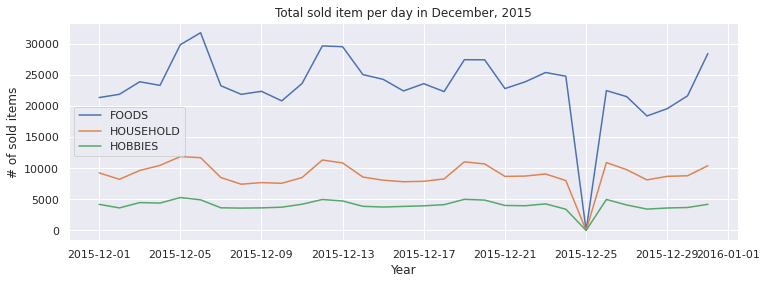
\includegraphics[width=0.8\linewidth]{img/totalSoldItemPerDayDec2015.png}
  \end{center}
    \caption{Total items sold per day in December 2015.\cite{ryuheeeei_2020}}
  \label{fig:totalSoldItemPerDayDec2015}
\end{figure*}
  Figure~\ref{fig:totalSoldItemPerDayDec2015} shows the sales for the month of
  December in 2015. Here it shows that the day of the drop is December 25 which
  is Christmas Day.

\begin{figure*}
  \begin{center}
    % \fbox{\rule{0pt}{2in} \rule{.9\linewidth}{0pt}}
    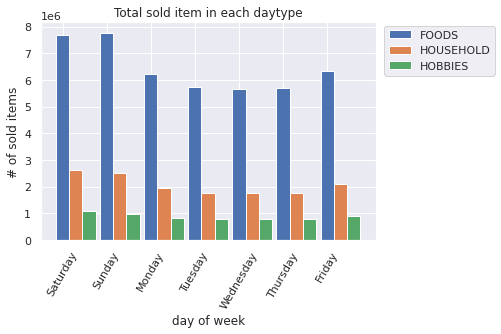
\includegraphics[width=0.8\linewidth]{img/totalSoldItemInEachDayOfWeek.png}
  \end{center}
    \caption{Total items sold each day of the week. \cite{ryuheeeei_2020}}
  \label{fig:totalSoldItemInEachDayOfWeek}
\end{figure*}
  Figure~\ref{fig:totalSoldItemInEachDayOfWeek} shows the number of items sold
  per day of the week. Here we can see how people tend to do grocery shopping on
  weekends and sales are lower towards the middle of the week. This correlates
  to many stores doing restock on Tuesdays.

\begin{figure*}
  \begin{center}
    % \fbox{\rule{0pt}{2in} \rule{.9\linewidth}{0pt}}
    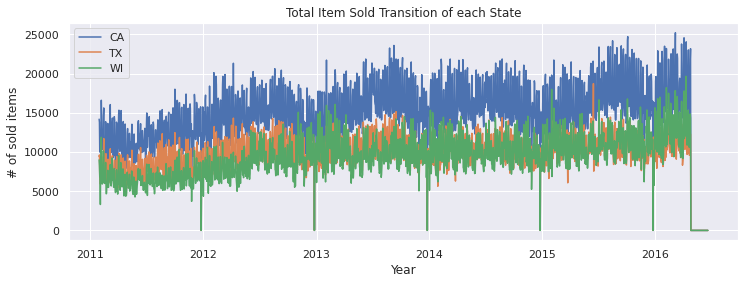
\includegraphics[width=0.8\linewidth]{img/totalItemSoldInEachState.png}
  \end{center}
    \caption{Total items sold in each state.\cite{ryuheeeei_2020}}
  \label{fig:totalItemSoldInEachState}
\end{figure*}
  Lastly, Figure~\ref{fig:totalItemSoldInEachState} graphs the items sold in
  California, Texas and Wisconsin showing, as we should expect, that a bigger
  population means more sales.

%-------------------------------------------------------------------------
\section{Approach}
% Background tutorial (if necessary)
% Your technical innovation (might be multiple pages/sections, with repeated reference to scientific gap)
  The approach corresponds with the files attached to the BlackBoard submission,
  which contains all the source code used to generate files, train, and run
  evaluation on.

\subsection{Dataset}
  In order to train a Neural Network that can learn to correctly predict the
  number of sales per the hierarchical data shown above, i.e. item in a
  department, in a particular store, in a particular state, for a particular
  range of dates, we collapsed the star schema into a singular table containing
  all this information, with the dates and corresponding sales both
  becoming respondent columns. The training file ended up looking as such.

\noindent {\bf sales.csv} - training file for the neural network, containing
labels and its respective metadata.

{\small\begin{verbatim}
schema: sales, id, item_id, dept_id, cat_id,
        store_id, state_id, d, date,
        wm_yr_wk, weekday, wday, month,
        year, event_name_1, event_type_1,
        event_name_2, event_type_2, snap_CA,
        snap_TX, snap_WI, sell_price

row: 0, HOBBIES_1_001_CA_1_validation,
     HOBBIES_1_001, HOBBIES_1, HOBBIES, CA_1,
     CA, d_1, 2011-01-29, 11101, Saturday, 1,
     1, 2011, , , , , 0, 0, 0,
\end{verbatim}}


The column sales correspond to the number of products sold at that certain date
per the hierarchical item. In order to develop such a training set, it is
necessary to check for the correctness of data. We made sure there are no
duplicate columns or rows, and that all data was filled correctly for a proper
merge operation between the respective fields across the tables. All the joins
were done using outer joins, so incoming results had missing fields such as a
pricing per item at a particular date.

 The sales\_train\_validation.csv contained 30490 entries, however, with the
sales.csv having rolled out the dates into columns of their own, and having
merged with its surrounding tables, it became over 60 million rows, a job for a
server computer with at least 50GB of RAM. At the time, we didn't have access to
a server computer, therefore we partitioned the data and then concatenated it
together. Once we had access to a server computer with 128GB of RAM, we were
able to load the dataset into memory. Loading the file into a Pandas' dataframe
took over 4 minutes. However, after manually typing the Pandas' columns to
smaller data types, the loading time decreased to an estimated 3-4 minutes. The
types were define as shown on Table \ref{typesTable}

\begin{table}[]
  \begin{center}
    \begin{tabular}{|l|l|}
      \hline
            Column Name & Type \\
      \hline\hline
      snap\_CA & int8 \\
      snap\_TX & int8 \\
      snap\_WI & int8 \\
      sales & float32 \\
      wm\_yr\_wk & int16 \\
      wday & int8 \\
      month & int8 \\
      year & int8 \\
      sell\_price & float32 \\
      \hline
    \end{tabular}
  \end{center}
  \label{typesTable}\
  \caption{Types Table.}
\end{table}


\subsection{Model/Data}
The model we used was a tabular model from a popular repository on
GitHub~\cite{fastai_2020}, https://github.com/fastai/fastai. The underlying
details worked as in the corresponding manner: first, we defined the dataset to
be fed to the model as a TabularDataBunch, which is a hierarchical abstraction
to the Dataloader and Dataset classes and manipulation as given in PyTorch for
tabular datasets. It bunches the data up to be trained upon, customized, and
assists with preprocessing. Our sales.csv conformed to what was specified by the
PyTorch API and was loaded successfully. The DataBunch API allowed us to fill in
the previously mentioned data such as pricing, by using the median of the values
across the column. We also normalize the pricing column using standardization.
The prices ranged from \$0.01 to \$107.32, before standardization.

\begin{quote}
  \begin{equation}
    Z=\frac{x-u}{\phi}
    \label{newEquatation}
    \cite{stephanie_2019}
  \end{equation}
  $Z$ = standard score

  $x$ = observed value

  $u$ = mean of the sample

  $\phi$ = standard deviation of the samples
\end{quote}

  The model uses embeddings under the hood in order to learn meaningful vectors
  for categorical variables during training that can be referenced during
  evaluations. Then subsequent layers are defined to learn the interaction
  between these embeddings and the dependent variable, i.e. sales. It contains
  BatchNorm layers to speed up training as well as adding an extra layer against
  overfitting, and a ReLU layer for nonlinearity. The dropout rate can be
  specified for both embeddings and the subsequent layers.

  Embeddings can have a vector size associated with them, and this is defined
  from a heuristic that the authors seem to have come up with through empirical
  means. The embeddings also have an extra size to their number of categories,
  in order to have another vector for an unknown field that is encountered, i.e.
  \#na.

  Below is a view of the model of the best results from our Kaggle submissions,
  as we have tried increasing the layers on the model to no avail, perhaps due
  to the limited training time we had. Again, the Embeddings are for our
  categorical variables + \#na, whereas our only continuous variable
  ‘sell\_prices' is fed in as the normalized value directly. The method to do it
  is that in the forward pass of the model, it takes all the vectors of the
  embeddings, flattens them into one vector, then appends the continuous
  variable to the end of the value, thus having a single vector as input to the
  subsequent layers.

{\scriptsize
\begin{verbatim}
TabularModel(
  (embeds): ModuleList(
    (0): Embedding(6, 4)
    (1): Embedding(2, 2)
    (2): Embedding(2, 2)
    (3): Embedding(2, 2)
    (4): Embedding(2, 2)
    (5): Embedding(1532, 97)
    (6): Embedding(8, 5)
    (7): Embedding(8, 5)
    (8): Embedding(13, 7)
    (9): Embedding(6, 4)
    (10): Embedding(31, 11)
    (11): Embedding(5, 4)
    (12): Embedding(5, 4)
    (13): Embedding(3, 3)
    (14): Embedding(3, 3)
    (15): Embedding(3, 3)
    (16): Embedding(3, 3)
    (17): Embedding(3, 3)
  )
  (emb_drop): Dropout(p=0.04,
                      inplace=False)
  (bn_cont): BatchNorm1d(1,
                         eps=1e-05,
                         momentum=0.1,
                         affine=True,
                         track_running_stats=True)
  (layers): Sequential(
    (0): Linear(in_features=165,
                out_features=1000,
                bias=True)
    (1): ReLU(inplace=True)
    (2): BatchNorm1d(1000,
                     eps=1e-05,
                     momentum=0.1,
                     affine=True,
                     track_running_stats=True)
    (3): Dropout(p=0.001,
                 inplace=False)
    (4): Linear(in_features=1000,
                out_features=500,
                bias=True)
    (5): ReLU(inplace=True)
    (6): BatchNorm1d(500,
                     eps=1e-05,
                     momentum=0.1,
                     affine=True,
                     track_running_stats=True)
    (7): Dropout(p=0.01, inplace=False)
    (8): Linear(in_features=500,
                out_features=1,
                bias=True)
  )
)
\end{verbatim}
}

\subsection{Loss Functions/Forward Methods}
There were two different options for the Forward functions. We tried both.
\begin{enumerate}
  \item A simple output through the layers of the neural network, with no
  modifications to the output variable.
  \item A squashed and re-expanded output by means of using the sigmoid function
  with a specified dependent variable range.
\end{enumerate}
  A simple output through the layers of the neural network, with no
  modifications to the output variable.

\begin{equation}
  (y_1 - y_0) * sigmoid(x) + y_0
  \label{newEqn}
\end{equation}

  This method is particularly useful when you are more interested in ratios of
  the output being close to each other, especially when paired with a method of
  logging the dependent variable and inverting the logging for submission.
  However, the mean(1.0312) and scale(0-763) of the dependent variable was not
  appropriate for this forward pass. The intuition is that the Sigmoid function
  tends to saturate towards 0 and 1, and having outliers that raises the scale
  makes it a harder task for the Neural Network. The results, as will be
  discussed in the Results/Extras section demostrate this.

  The loss for both forward passes is a Mean Squared Error Loss function.

  \begin{equation}
    MSE = \frac{1}{n}\sum_{i=1}^{n} (y_i - \hat{y_i})^2
    \label{newEqn}
  \end{equation}

  This is typical of regression tasks which tries to minimize the residual sum
  of squares.

  The metric used in the paper is Weighted Root Mean Squared Scaled Error
  (RMSSE), however in terms of training, it’s fine to use a MSE.

\subsection{Training}
  Training the Neural Network can be a tedious task, with iterative and manual
  methods to try and converge the train/valid/test losses down to zero. However,
  we took a much more scientific approach as given from the API of fastai. We
  used a learning rate finder algorithm, which employs a callback while
  increasing the learning rate, to see when the losses would diverge. Then we
  take the learning rate right before the diversion, and scale it down by the
  desired factor and choose that as the learning rate. For larger datasets per
  epoch, e.g. $>$ 60 million entries, one might choose the far left of the
  graph, whereas in regular cases it’s recommended to scale down by a factor of
  10-100.

  \begin{figure}[]
    \centering
    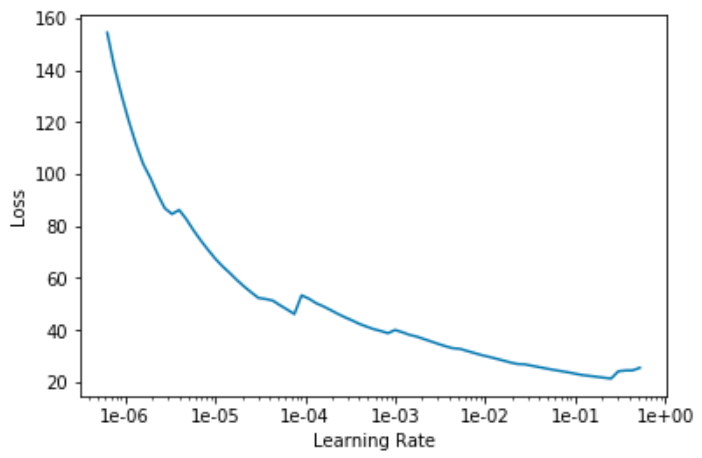
\includegraphics[width=0.8\linewidth]{img/learningRate.png}
    % \caption{}
    \label{learningRate}
  \end{figure}

  For the actual SGD process, we used a fit one-cycle method on top of the Adam
  Optimizer. The Adam Optimizer from PyTorch was given betas of (.95, .99) for
  the calculation of moving averages of the gradients, and the default epsilon
  value of 1e-08 to the denominator for numerical stability. The more
  interesting piece is the fit one-cycle method which helps a bit in
  regularization, finding a better optima, as well as speeding up training. The
  method is to raise a learning rate to the maximum value we found through the
  learning rate finder, and then decrease it throughout one cycle. The graph of
  the learning rate throughout its course resembles that of cosine annealing. In
  parallel, as the learning rate shifts, an inverse shift happens to the
  momentum, in order to not tack on too much at the high levels of the learning
  rate curve and gradually let it pick up enough during the transition to the
  lower learning rate. When the learning rate peaks, it can throw the neural
  network out of local maximas, due to some parts of the parameter having
  possibly diverged, and then when the learning rate anneals down, the network
  zones in to converge to what’s hopefully a good medium. We found running two
  cycles with 1 epoch each worked best, since each epoch contained too many
  iterations and found keeping the learning rate high for too long made the
  network a bit less optimal.

  Each epoch took roughly 4-5 hours to run.

  The training was done for different sets of hyper parameters and tweaks, as
  shown under Results/Trials.


%-------------------------------------------------------------------------
\section{Results/Trials}
% Data sets, simulator, implementation details
% Empirical results (might be multiple pages)
  We have tagged our different set of models to a unique identifier. Each model
  in each category was trained atop the previous natural ordered model, e.g.
  second.pth was trained after loading first.pth and b2high.pth was trained
  after having loaded b2.pth.

\begin{table}[]
  \begin{center}
    \begin{tabular}{|l|l|l|l|}
    \hline
                      & first.pth & second.pth & third.pth \\ \hline
    Learning Rate     & 1e-5      & 1e-7       & 1e-9      \\ \hline
    Epochs            & 1         & 1          & 1         \\ \hline
    WD                & 0.1       & 0.1        & 0.1       \\ \hline
    Results on Kaggle & 5.36372   & 5.18228    & 5.32621   \\ \hline
    Train Loss        & 13.502676 & 13.329883  & 12.989215 \\ \hline
    Valid Loss        & 19.568241 & 19.618902  & 19.616224 \\ \hline
    \end{tabular}
    {\scriptsize
    \begin{verbatim}
Linear Layers: (165, 1000), (1000, 500), (1000,250), (250, 1)
Respective dropouts: 0.05, 0.1, 0.2
Embedding dropout: 0.1
    \end{verbatim}}
  \end{center}
  \caption{Models with labels that we applied the log function to, then inverse
  at evaluation/submission time.}
\end{table}

\begin{table}[]
  \begin{center}
    \begin{tabular}{|l|l|l|}
    \hline
                      & a1.pth   & a2.pth   \\ \hline
    Learning Rate     & 1e-6     & 1e-7     \\ \hline
    Epochs            & 1        & 1        \\ \hline
    WD                & 0.1      & 0.1      \\ \hline
    Results on Kaggle & 1.44203  & 0.94467  \\ \hline
    Train Loss        & 6.295133 & 5.254736 \\ \hline
    Valid Loss        & 7.124599 & 8.201993 \\ \hline
    \end{tabular}
    {\scriptsize
    \begin{verbatim}
Linear Layers: (165, 1000), (1000, 500), (500, 1)
Respective dropouts: 0.001, 0.01
Embedding dropout: 0.04
    \end{verbatim}}
  \end{center}
  \caption{Models with labels left as is.}
\end{table}

\begin{table}[]
  \begin{center}
    \begin{tabular}{|l|l|l|}
    \hline
                      & b1.pth   & b2.pth   \\ \hline
    Learning Rate     & 1e-6     & 1e-8     \\ \hline
    Epochs            & 1        & 1        \\ \hline
    WD                & 0.1      & 0.1      \\ \hline
    Results on Kaggle & 1.37687  & 1.16362  \\ \hline
    Train Loss        & 7.605392 & 6.114019 \\ \hline
    Valid Loss        & 7.048354 & 7.206628 \\ \hline
    \end{tabular}
    {\scriptsize
    \begin{verbatim}
Linear Layers: (165, 1000), (1000, 500), (1000,250), (250, 1)
Respective dropouts: 0.05, 0.1, 0.2
Embedding dropout: 0.1
    \end{verbatim}}
  \end{center}
  \caption{Models with labels left as is.}
\end{table}

\begin{table}[]
  \begin{center}
    \begin{tabular}{|l|l|l|l|}
    \hline
                      & k1.pth  & p.pth   & p1.pth  \\ \hline
    Learning Rate     & 1e-6    & 1e-5    & 1e-5    \\ \hline
    Epochs            & 1       & 1       & 1       \\ \hline
    WD                & 0.1     & 0.1     & 0.1     \\ \hline
    Results on Kaggle & 6.23465 & 5.36372 & 5.36372 \\ \hline
    \end{tabular}
  \end{center}
  \caption{Models using the sigmoid * range forward function Same layer,dropout
  setting as previous, however k1.pth scaled the max dep var to be ½ of actual
  max}
\end{table}


%-------------------------------------------------------------------------
\section{Related Work}
% Dont just say whats been done. Point out how prior work relates to yours and to the scientific gap you set forth in the intro.
The relate work goes here

%-------------------------------------------------------------------------
\section{Summary/Discussion/Conclusion}
% Summary problem, approach, result, in past tense
% Discuss open questions, promising research directions
The Summary Goes here








% %-------------------------------------------------------------------------
% \section{\LaTeX\ Reference Section}
% \verb'\cvprfinalcopy' Is for different font

% (e.g.\ this line is $095.5$)

% An example of a bad paper:
% \begin{quote}
% \begin{center}
%     An analysis of the frobnicatable foo filter.
% \end{center}

%    In this paper we present a performance analysis of our
%    previous paper [1], and show it to be inferior to all
%    previously known methods.  Why the previous paper was
%    accepted without this analysis is beyond me.

%    [1] Removed for blind review
% \end{quote}

% This is how you cite a reference submission~\cite{Authors06} as additional material and

% \begin{quote}
% and this is a quote and a another special formatting {\tt eccv06.pdf}.
% \end{quote}

% {\em require} more special formatting

% ``Zero-g frobnication: How being the only people in the world with access to
% the Apollo lander source code makes us a wow at parties'', by Zeus \etal.

% FAQ: Are acknowledgements OK?  No.  Leave them for the final copy.


% \begin{figure}[t]
%   \begin{center}
%     \fbox{\rule{0pt}{2in} \rule{0.9\linewidth}{0pt}}
%     % 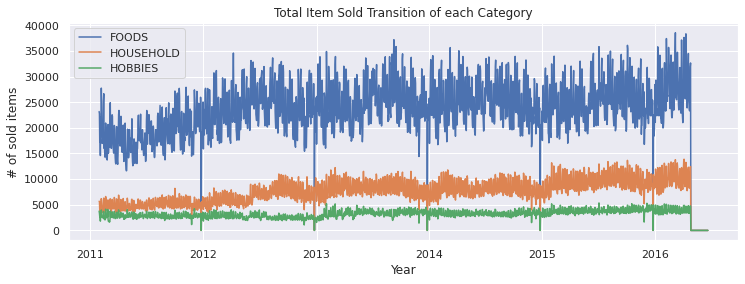
\includegraphics[width=0.8\linewidth]{img/meh.png}
%   \end{center}
%     \caption{Example of caption.  It is set in Roman so that mathematics
%     (always set in Roman: $B \sin A = A \sin B$) may be included without an
%     ugly clash.}
%   \label{fig:long}
%   \label{fig:onecol}
% \end{figure}

% \noindent
% Compare the following:\\
% \begin{tabular}{ll}
%  \verb'$conf_a$' &  $conf_a$ \\
%  \verb'$\mathit{conf}_a$' & $\mathit{conf}_a$
% \end{tabular}\\
% See The \TeX book, p165.

% The space after \eg, meaning ``for example'', should not be a
% sentence-ending space. So \eg is correct, {\em e.g.} is not.  The provided
% \verb'\eg' macro takes care of this.

% When citing a multi-author paper, you may save space by using ``et alia'',
% shortened to ``\etal'' (not ``{\em et.\ al.}'' as ``{\em et}'' is a complete word.)

% For this citation style, keep multiple citations in numerical (not
% chronological) order, so prefer \cite{Alpher03,Alpher02,Authors06} to
% \cite{Alpher02,Alpher03,Authors06}.





% This is fractions text area is $6\frac78$ inches (17.5 cm) wide by $8\frac78$
% and more $\frac{5}{16}$ and other $8.5 \times 11$-inch

% Reference figurers Figures~\ref{fig:onecol} and~\ref{fig:short}.  Short captions should be centred.

% \noindent For no indent

% FIRST-ORDER HEADINGS. (For example, {\large \bf 1. Introduction})

% SECOND-ORDER HEADINGS. (For example, { \bf 1.1. Database elements})

% Please use footnotes\footnote {This is what a footnote looks like.  It
% often distracts the reader from the main flow of the argument.} sparingly.

% \begin{table}
%   \begin{center}
%     \begin{tabular}{|l|c|}
%       \hline
%       Method & Frobnability \\
%       \hline\hline
%       Theirs & Frumpy \\
%       Yours & Frobbly \\
%       Ours & Makes one's heart Frob\\
%       \hline
%     \end{tabular}
%   \end{center}
%   \caption{Results.   Ours is better.}
% \end{table}

% When placing figures in \LaTeX, it's almost always best to use
% \verb+\includegraphics+, and to specify the  figure width as a multiple of
% the line width as in the example below
% {\small\begin{verbatim}
%    \usepackage[dvips]{graphicx} ...
%    \includegraphics[width=0.8\linewidth]
%                    {myfile.eps}
% \end{verbatim}
% }


{\small
\bibliographystyle{ieee}
\bibliography{egbib}
}

\end{document}
